\documentclass[aspectratio=1610]{beamer}
\usetheme{Madrid}


\usepackage{amsmath}
\usepackage{amssymb}
\usepackage{listings}
\usepackage{booktabs}
\usepackage{multirow}
\usepackage{multirow}
\usepackage{lmodern}
\usepackage{xcolor}
\usepackage{float}
\lstset{
  language=Python,  %代码语言使用的是matlab
  % frame=shadowbox, %把代码用带有阴影的框圈起来
  rulesepcolor=\color{red!20!green!20!blue!20},%代码块边框为淡青色
  keywordstyle=\color{blue!90}\bfseries, %代码关键字的颜色为蓝色,粗体
  commentstyle=\color{red!10!green!70}\textit,    % 设置代码注释的颜色
  basicstyle=\footnotesize,
  showstringspaces=true,%不显示代码字符串中间的空格标记
  % numbers=left, % 显示行号
  % numberstyle=8pt,    % 行号字体
  % numberstyle=\color{green},
  stringstyle=\rmfamily\slshape\color[RGB]{128,0,0}, % 代码字符串的特殊格式
  breaklines=true, %对过长的代码自动换行
  extendedchars=false,  %解决代码跨页时,章节标题,页眉等汉字不显示的问题
  escapeinside=``,%代码中出现中文必须加上,否则报错
  texcl=true}

\lstset{breaklines}%自动将长的代码行换行排版

\lstset{extendedchars=false}%解决代码跨页时,章节标题,页眉等汉字不显示的问题

\usepackage{textcomp}
% \usepackage[margin=1in]{geometry}
\usepackage{pythonhighlight}
% \usepackage{minted}
\usepackage[backend=bibtex]{biblatex}
%\usepackage[style=authortitle,backend=biber]{biblatex}
\addbibresource{ResearchRabbit_Export_2022_10_20.bib}

\usepackage{algorithm}
\usepackage{algorithmic}
\renewcommand{\algorithmicrequire}{\textbf{Input:}}
\renewcommand{\algorithmicensure}{\textbf{Output:}}


\title[logic synthesis libraries]{The EPFL Logic Synthesis Libraries}
\author[Gcc]{Dingchao Gao}
\institute[ISCAS]{Institute of Software Chinese Academy of Sciences}

\begin{document}

\begin{frame}[plain]
  \titlepage
  %  Title page
\end{frame}

\section{induction}
\begin{frame}
  SIS, 
\end{frame}

<<<<<<< Updated upstream
\section{flow algorithm}
=======
\begin{frame}{quantum libraries}
  \begin{itemize}
    \item angel: quantum state preparation library
    \item tweedledum: quantum compilation library
    \item caterpillar: quantum circuit synthesis library
  \end{itemize}
\end{frame}
>>>>>>> Stashed changes
\begin{frame}{initial state \footfullcite{initial}}
    \begin{itemize}
      \item target:
      \begin{align}
        \left|\varphi_{j}\right\rangle= \frac{1}{\sqrt{|on(f)|}} \sum_{x \in \operatorname{on}(f)}|x\rangle
      \end{align}
      \item the  general  idea  of  state  preparation  algorithm  relies on the identity:
      \begin{align}
        \mathrm{QSP}_{f}|0\rangle^{\otimes n} = \left(\mathrm{QSP}_{f_{\bar{x}_{i}}} \oplus \mathrm{QSP}_{f_{x_{i}}}\right)\left(G\left(p_{f}\left(\bar{x}_{i}\right)\right) \otimes I_{2^{n}-1}\right)|0\rangle
      \end{align}
      \item $G\left(p_{f}\left(\bar{x}_{i}\right)\right)$ is a unitary transformation gate that satisfies:
      \begin{align}
        G(p_{f}\left(\bar{x}_{i}\right))|0\rangle = \sqrt{p_{f}\left(\bar{x}_{i}\right)}|0\rangle+\sqrt{1-p_{f}\left(\bar{x}_{i}\right)}|1\rangle
      \end{align}
      \begin{align}
        G\left(p_{f}\left(\bar{x}_{i}\right)\right) = R_{y}\left(2 \cos ^{-1}\left(\sqrt{p_{f}\left(\bar{x}_{i}\right)}\right)\right)
      \end{align}
    \end{itemize}
  \end{frame}
  \begin{frame}
    \begin{figure}[htbq]
      \centering
      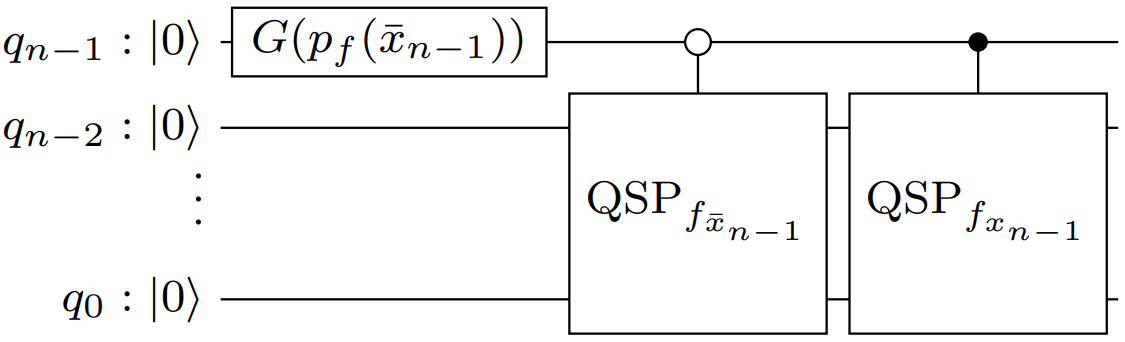
\includegraphics[width=0.9\textwidth]{figure/QSP.png}
      \caption{the general idea of QSP in the quantum  circuit  model for $i=n-1$.} 
      \label{fig-qsp}
    \end{figure}
  \end{frame}
  \begin{frame}{initial state example}
    \begin{figure}[htbq]
      \centering
      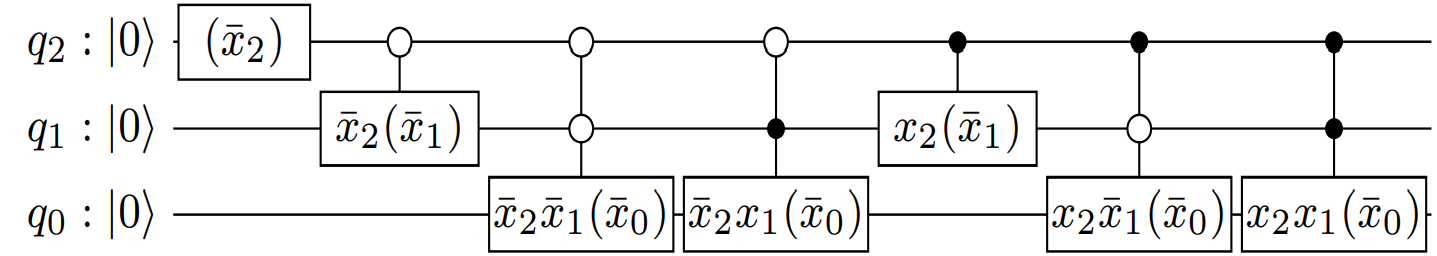
\includegraphics[width=0.9\textwidth]{figure/qsp_example.png}
      \caption{the abstract quantum gates of $QSP_{<x_0x_1x_2>}$} 
      \label{fig-qsp-example}
    \end{figure}
  \end{frame}
  \begin{frame}
    \begin{figure}[htbq]
      \centering
      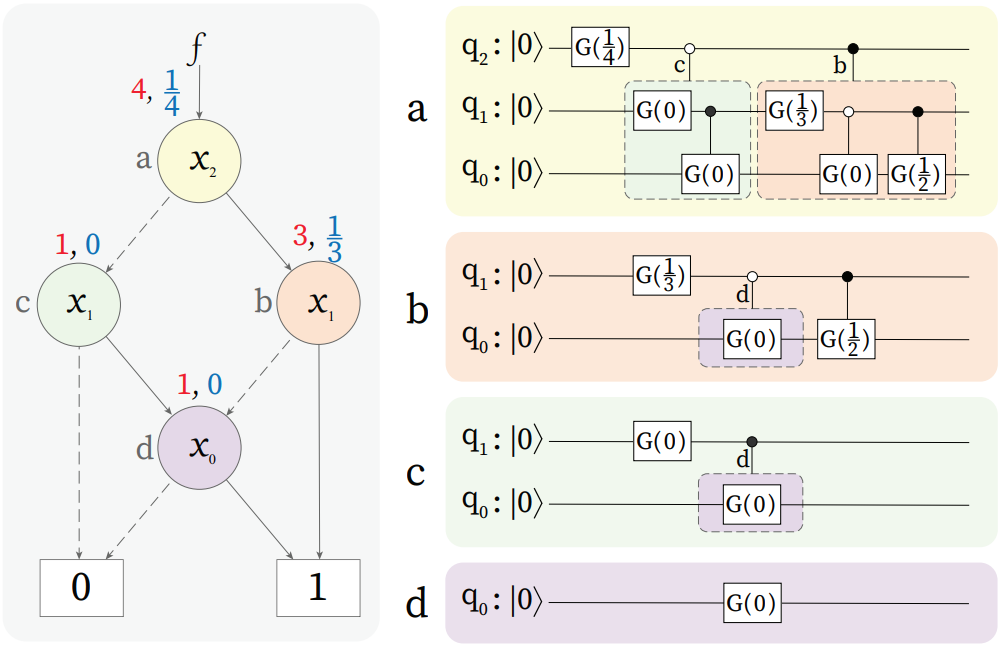
\includegraphics[width=0.8\textwidth]{figure/qsp_circuit.png}
      \caption{BDD  for boolean function $f= x_0x_1\vee x_1x_2 \vee x_2x_0 $ and  the  procedure  of  extracting  gates  for  each node from bottom to top} 
      \label{fig-qsp-example-circuit}
    \end{figure}
  \end{frame}
  \begin{frame}{compiling oracle by XAG\footfullcite{multiplicative}}
    \begin{itemize}
      \item representing an n-variable boolean function using a logic network over the gate basis$\{\lnot ,\oplus ,\wedge \}$:
      \begin{align}
        x_{i} = x_{j(i)} \oplus x_{k(i)} \quad \text { or } \quad x_{i} = x_{j(i)}^{p(i)} \wedge x_{k(i)}^{q(i)}
      \end{align}
      where $n< i \leq n+r$
      \item  the linear transitive fan-in of a node $x_i $using the recursive function:
      \begin{align}
        \operatorname{ltfi}\left(x_{i}\right) = \left\{\begin{array}{ll}
        \left\{x_{i}\right\} & \text { if } i < n \text { or } \circ_{i}  = \wedge, \\
        \operatorname{ltfi}\left(x_{j(i)}\right) \triangle \operatorname{ltfi}\left(x_{k(i)}\right) & \text { otherwise }
        \end{array}\right.
      \end{align}
    \end{itemize}
  \end{frame}
  \begin{frame}{XAG example}
    \begin{itemize}
      \item for $f(x)=x_1x_2\vee x_2x_3\vee x_3x_1$
      \item can be realized by the logic network: 
      \begin{align}
        x_{4} & = x_{1} \oplus x_{2}, & x_{5} & = x_{2} \oplus x_{3} \\
        x_{6} & = x_{4} \wedge x_{5}, & x_{7} & = x_{2} \oplus x_{6}
      \end{align}
      \item the linear transitive fan-in of a node:
      \begin{align}
        \operatorname{ltfi}\left(x_{4}\right) & = \left\{x_{1}, x_{2}\right\} 
        ,&\operatorname{ltfi}\left(x_{5}\right) & = \left\{x_{2}, x_{3}\right\} \\
        \operatorname{ltfi}\left(x_{6}\right) & = \left\{x_{6}\right\} 
        ,&\operatorname{ltfi}\left(x_{7}\right) & = \left\{x_{2}, x_{6}\right\} 
      \end{align}
    \end{itemize}
  \end{frame}
  
  \begin{frame}{XAG}
    \begin{columns}
      \begin{column}{0.48\linewidth}
        \begin{figure}[h]
          \centering
          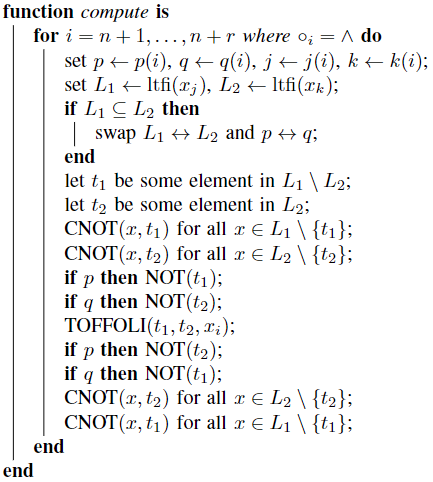
\includegraphics[width=0.8\textwidth]{figure/function.png}
          \label{fig-function}
        \end{figure}
      \end{column}
      \begin{column}{0.48\linewidth}
        \begin{figure}[h]
          \centering
          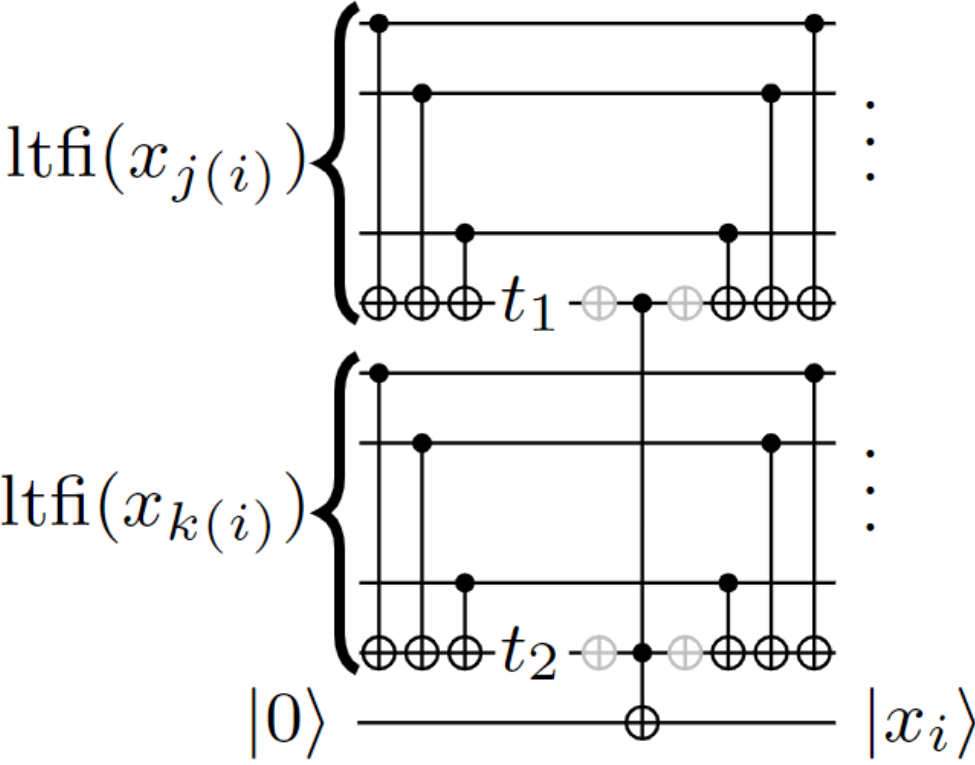
\includegraphics[width=0.4\textwidth]{figure/construction.png}
          \caption{quantum circuit construction for function compute}
          \label{fig-construction}
        \end{figure}
        \begin{algorithm}[H]
          \algsetup{linenosize=\tiny} \scriptsize
          \caption{Heuristic compilation algorithm} 
          \label{alg-be} 
          \begin{algorithmic}
            \REQUIRE Logic network with gates $x_{n+1}, \dots, x_{n+r}$
            \ENSURE Quantum circuit for $Uf$
            \STATE compute
            \STATE $\operatorname{CNOT}(x_{n+r-1},y)$
            \IF{p}
            \STATE $\operatorname{NOT}(y)$
            \ENDIF
            \STATE $compute^{\dagger}$
          \end{algorithmic} 
        \end{algorithm}
      \end{column}
    \end{columns}
  \end{frame}
  
  \begin{frame}{pebbling\footfullcite{Meuli_2019}}
    \begin{itemize}
      \item target: solving iteratively the reversible pebbling game on the given network
      \item method: the problem is encoded as a SAT problem and addressed by state-of-the-art solvers
      \item result: get the trade-off between qubits and operations
    \end{itemize}
  \end{frame}
  \begin{frame}{pebbling example}
    \begin{columns}
        \column{0.5\linewidth}
        \begin{minipage}[c][0.4\textheight][c]{\linewidth}
          \begin{figure}[h]
            \centering
            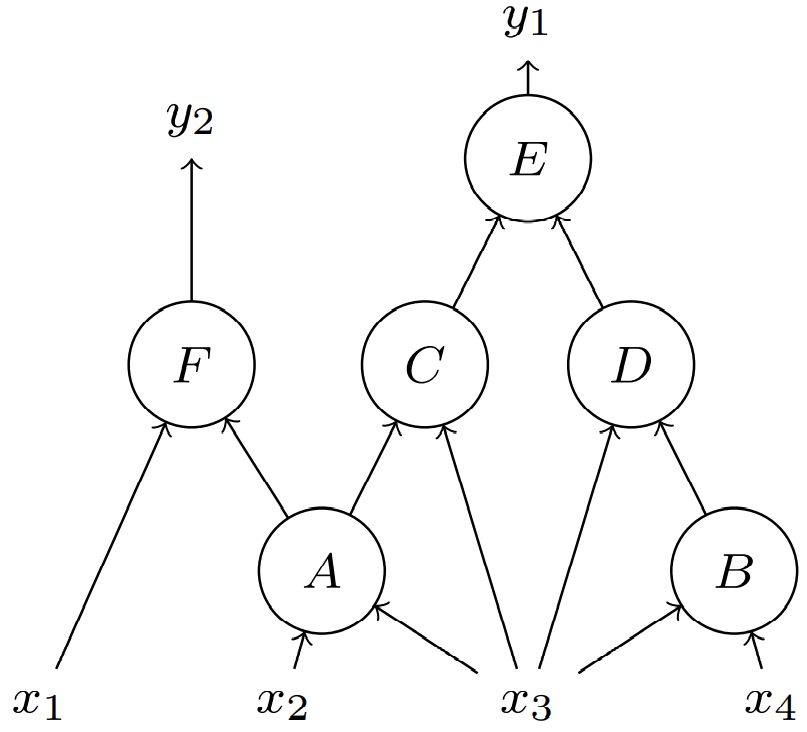
\includegraphics[width=0.4\textwidth]{figure/DAG.png}
            \caption{example of a directed acyclic graph}
          \end{figure}
        \end{minipage}
        \begin{minipage}[c][0.4\textheight][c]{\linewidth}
          \begin{figure}[h]
            \centering
            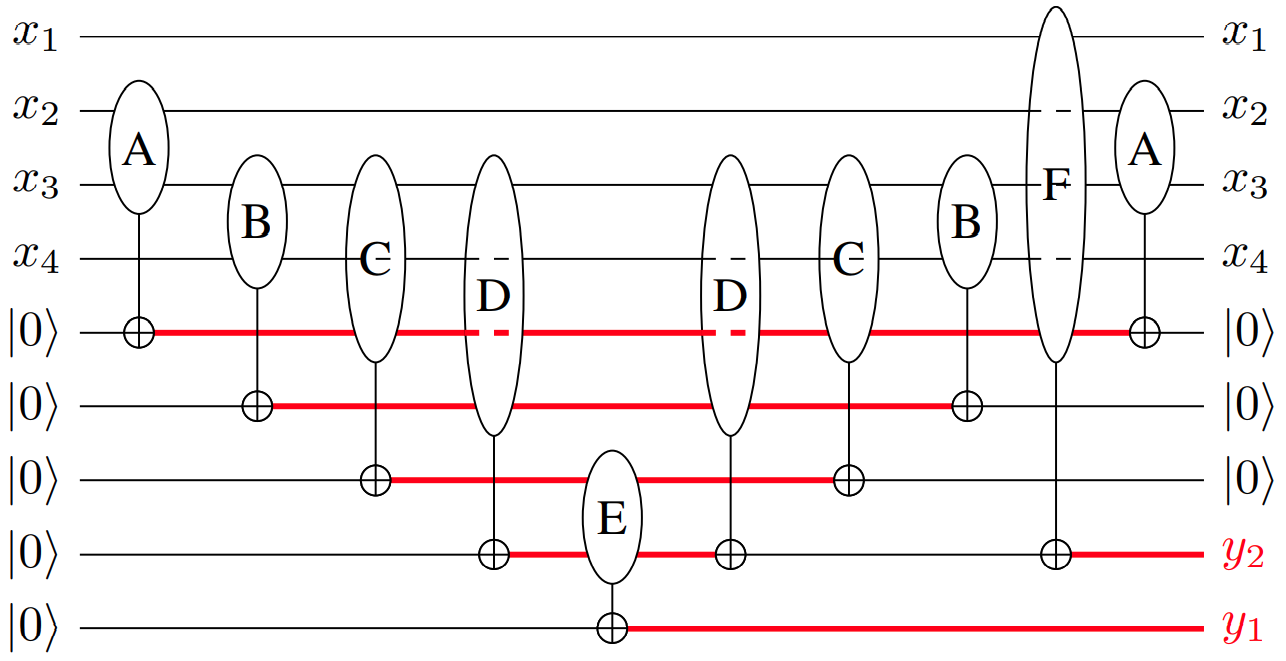
\includegraphics[width=0.8\textwidth]{figure/b.png}
            \caption{space-optimized by reordering}
          \end{figure}
        \end{minipage}
        
        \column{0.5\linewidth} % remember add this to the other clumn
        \begin{minipage}[c][0.4\textheight][c]{\linewidth}
          \begin{figure}[h]  
            \centering
            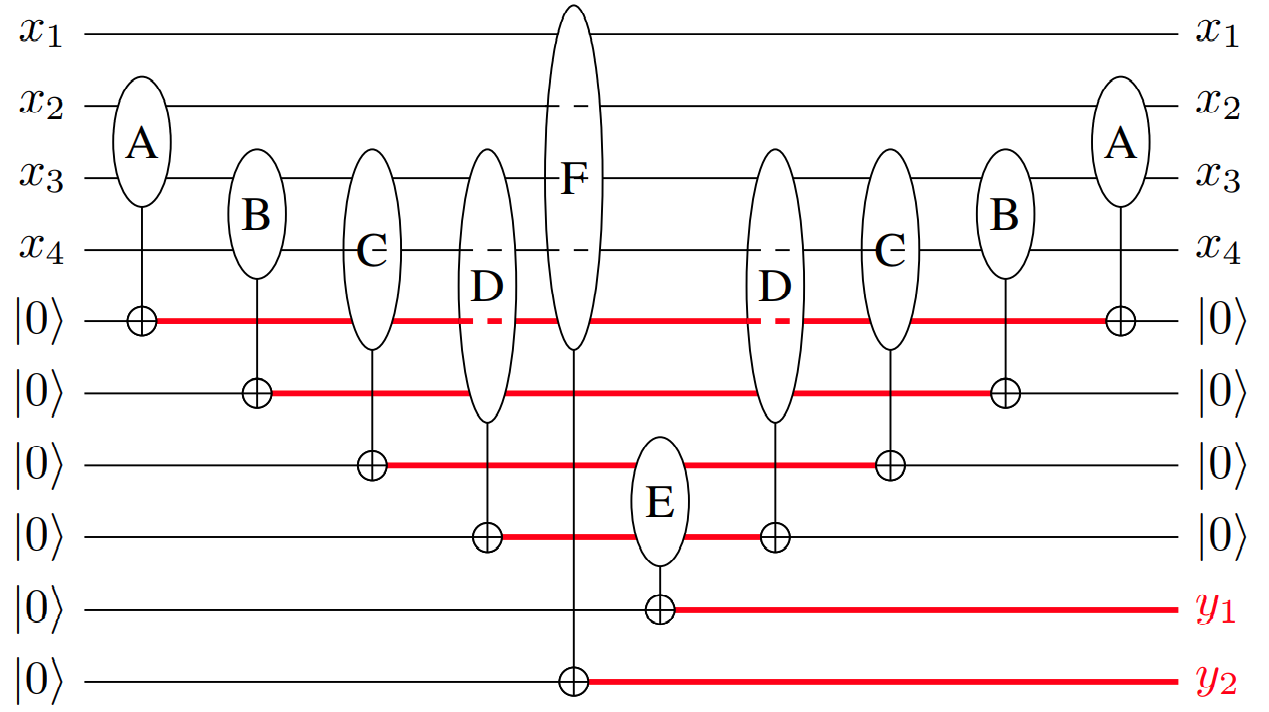
\includegraphics[width=0.6\textwidth]{figure/a.png}
            \caption{Bennet strategy}
          \end{figure}
      \end{minipage}
        \begin{minipage}[c][0.4\textwidth][c]{\linewidth}
          \begin{figure}[h]
              \centering
              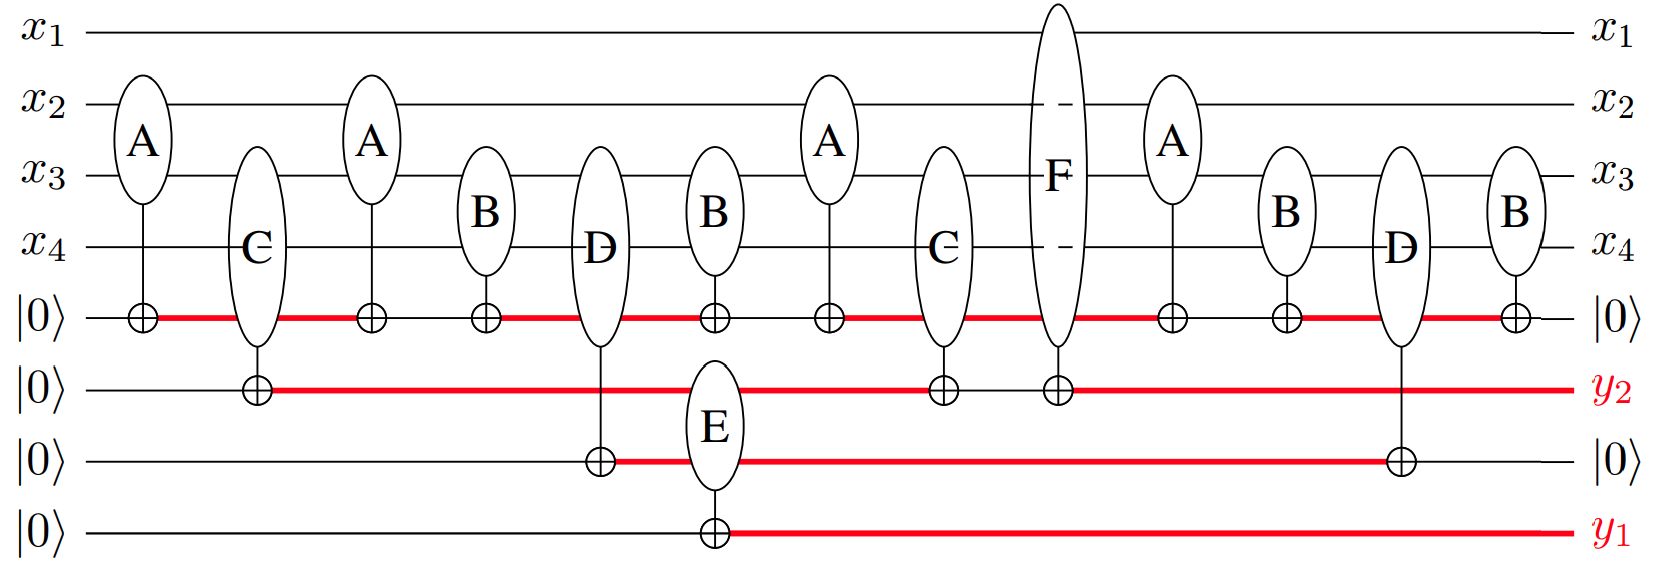
\includegraphics[width=0.8\linewidth]{figure/c.png}
              \caption{space-optimized by increasing the number of gates}
          \end{figure}
        \end{minipage}
    \end{columns}
  \end{frame}
\section{tweedledum}
\begin{frame}{induction}  
  ABC 
\end{frame}
\begin{frame}{compilation flow}
  \begin{figure}[htbq]
    \centering
    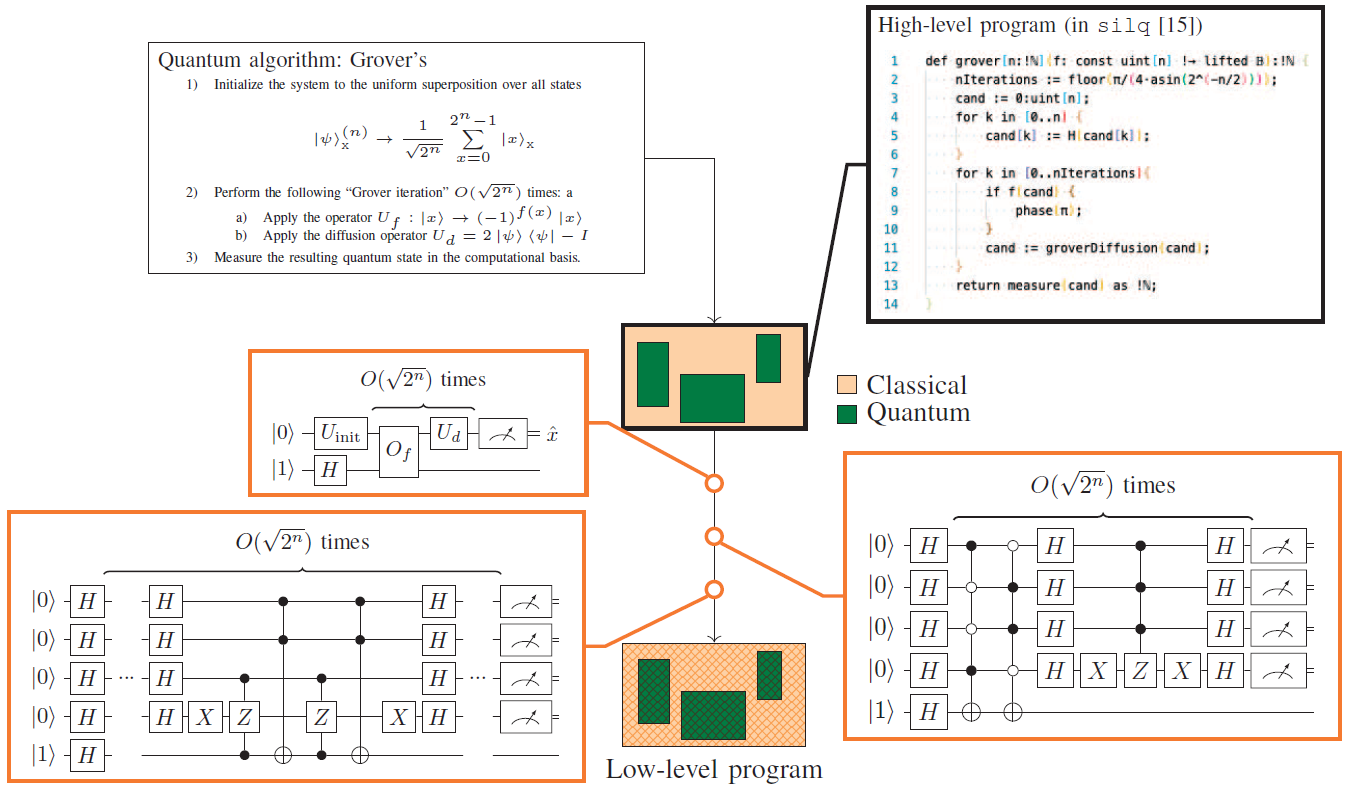
\includegraphics[width=0.8\textwidth]{figure/work_flow.png}
    \caption{compilation flow overview} 
    \label{fig-compilation}
  \end{figure}
\end{frame}
\begin{frame}{flexibility}
  \begin{figure}[htbq]
    \centering
    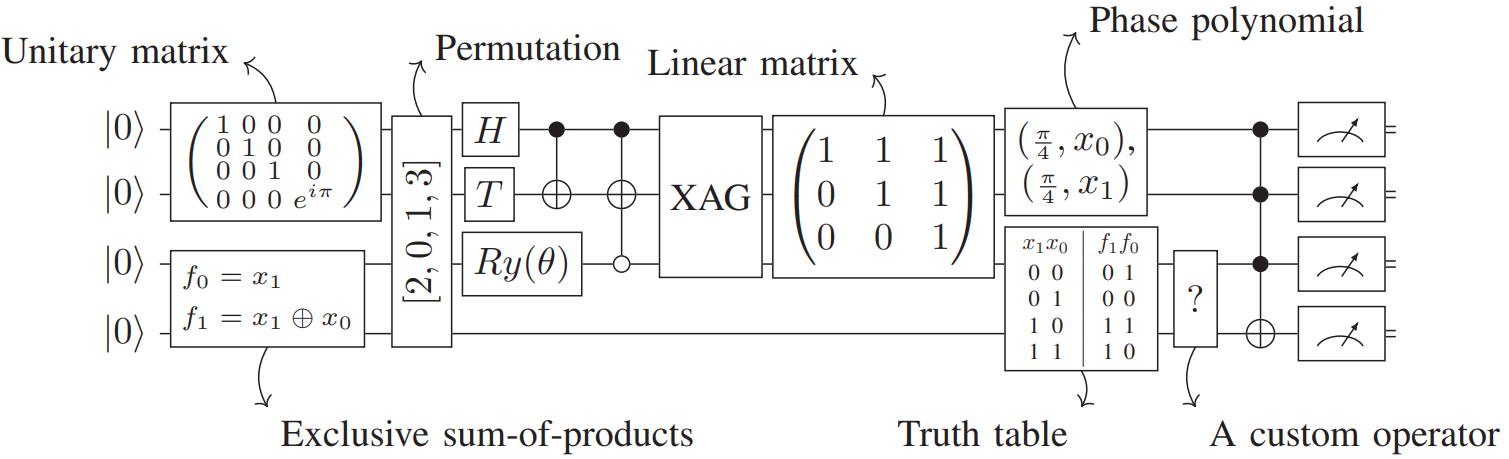
\includegraphics[width=0.9\textwidth]{figure/flex.png}
    \caption{tweedledum's IR flexibility} 
    \label{fig-flex}
  \end{figure}
\end{frame}
\begin{frame}{synthesis}
  \begin{itemize}
    \item 
  \end{itemize}  
\end{frame}
\begin{frame}{synthesis}
  \begin{figure}[htbq]
    \centering
    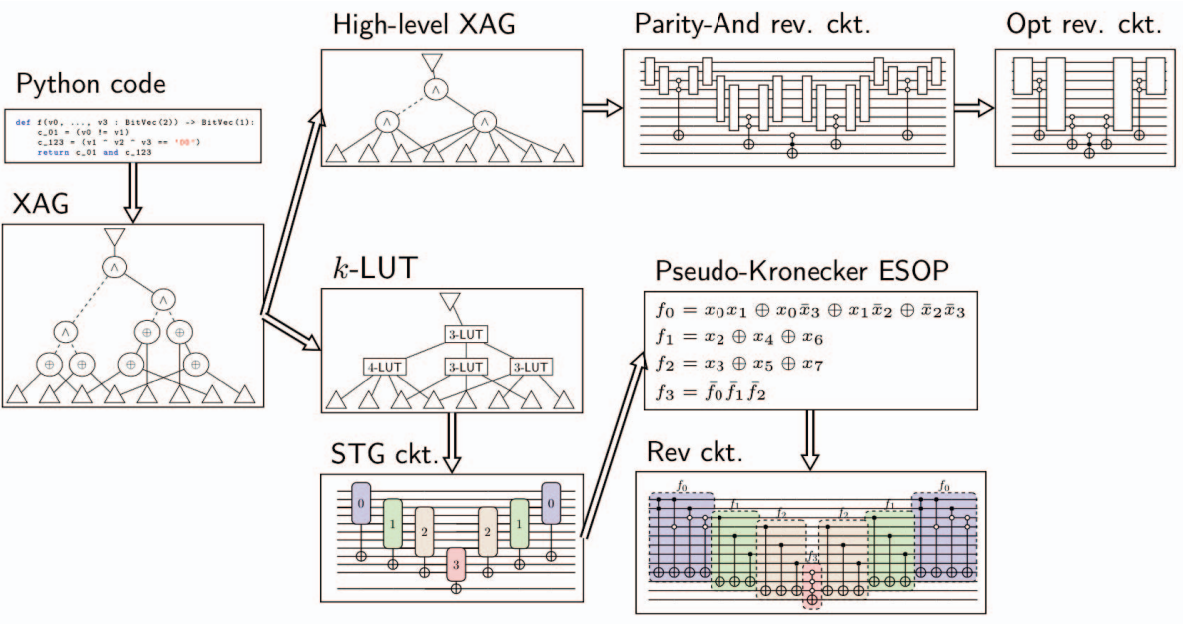
\includegraphics[width=0.7\textwidth]{figure/boolean.png}
    \caption{overview of possible Boolean function synthesis flows} 
    \label{fig-boolean}
  \end{figure}
\end{frame}
\begin{frame}{compilation passes}
  \begin{itemize}
    \item 
  \end{itemize}
\end{frame}

\section{Protocol Example}
\subsection{a protocol of leader in network}
\subsection{loop}

\begin{frame}{disscussion}
  \begin{itemize}
    \item lack of quantum computing features
    \item comparing with isq etc
    \item the abstract level of quantum computer? 
  \end{itemize}
\end{frame}
\begin{frame}{disscussion}
  \begin{figure}
    \centering
    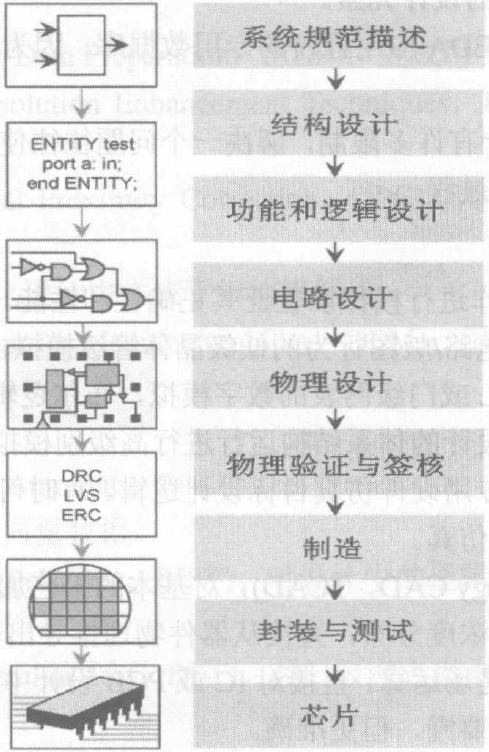
\includegraphics{figure/eda_flow.png}
    \caption{the main flow of ultra-large scale IC product design}
  \end{figure}
\end{frame}
\begin{frame}[noframenumbering,allowframebreaks,t]
	\frametitle{references}
	\printbibliography
\end{frame}

\begin{frame}
\centering
\Huge{END\\Thank you}
\end{frame}
\end{document}